%!TEX root = ../main.tex
%=========================================================

\section{Performance Evaluation}
\label{sec:eval}

In  this  section,  we  provide  a  detailed  investigation  of  the performance of the proposed discovery scheme.
We present the performance evalution in three different subsections. 
In the first one we evaluate the performance of our novel waiting function by measuring the ticket table occupancy
according with our design goals and parameters.
The second one is a thorough performance evaluation under different scenarios, including Sybil attacks, of the whole network discovery solution using a peer-to-peer network simulator.
%In the third one we include an evaluation using the most used Ethereum client software, Geth~\cite{go-ethereum}, in a testbed scenario.

\subsection{Ticket table occupancy evaluation}

\sergi{Ticket table occupancy and waiting time evaluation TBC}

\subsection{Network simulator evaluation}

\sergi{TODO: modify figures with bigger fonts}
\sergi{TODO: registrant distribution is not very readable. probably should be redesigned}
\sergi{TODO: Lookup performance should be compared with something. Discv4? }

%\subsubsection{Evaluation Setup}

For the network performance evaluation we extended the existing 
large-scale peer-to-peer network simulatior PeerSim~\cite{p2p09-peersim}.
We implemented the current Discv5 protocol by modyfing the available PeerSim Kademlia implementation with the differences of the Kademlia version used by the Ethereum network, and developing our solution on top of it. Our network simulator is available here\footnote{https://github.com/datahop/p2p-service-discovery}

In Table~\ref{tab:param} we show the parameters used in the simulation. 

\begin{table}[!hbt]
\centering
\scriptsize
\begin{tabular}{|c|c|}%|c|c|}
\hline
Parameter     & Value (\%) \\
\hline
\hline
%Network size & 2000 nodes \\%&  0.4321 & 0.8883\\
%\hline
Simulation time & 4 hours \\%& 0.7569 & 0.9959\\
\hline
Kademlia bucket size & 16 \\%& 0.6104 & 0.8515\\
\hline
Kademlia buckets & 17 \\%& 0.8225 & 0.9897\\
\hline
Ticket table bucket size & 5 \\%& 0.8225 & 0.9897\\
\hline
Ticket table buckets & 10 \\%& 0.8225 & 0.9897\\
\hline
Lookup table bucket size & 16 \\%& 0.8225 & 0.9897\\
\hline
Lookup table buckets & 17 \\%& 0.8225 & 0.9897\\
\hline
Registration lifetime & 15 minutes \\%& 0.8225 & 0.9897\\
\hline
Number of topics & 5 \\%& 0.8225 & 0.9897\\
\hline
Number of topics & 5 \\%& 0.8225 & 0.9897\\
\hline
Zipf dist exp & 0.7 \\%& 0.8225 & 0.9897\\
\hline
Ticket table capacity & 500 \\
\hline
Turbulence event & Every 144 seconds per 1000 nodes. \\%& 0.8225 & 0.9897\\
\hline
Num of connections & 50 \\%& 0.8225 & 0.9897\\
\hline
\bottomrule
\end{tabular}
\vspace{2mm}
\caption{Evaluation scenario parameters}
\label{tab:param}
\vspace{-0.05in}
\end{table}

We performed 4 hours long simulations with different number of nodes from 500 to 10000.
In the simulations there are 5 different topics and all nodes participate in at least one topic (t1).
There is turbulence in the simulation,  \ie new nodes are added to the network and existing nodes are removed at a rate of one event every 144 seconds per each thousand nodes in the network.
Nodes are modeled similarly to an Ethereum client. 
When a node joins the network it starts advertising for the participating topics.
Each node has a pool of connections (separated by outgoing and incoming connections) for each topic in which they participate, and it perform lookups
for a specific topic to start connections with discovered nodes.
When an initial lookup is done, the discovered nodes are stored in a buffer per topic.
Nodes start attempting connections with the discovered nodes from the buffer until all connections 
are full.
In case the connection is possible (the targeted node has an available slot in the pool of connections and the node is still up), it is added 
to the local list of connections.
Nodes are removed from the discovered nodes buffer for each attempt of connection.
When a node goes down, a connection attempt is maded with a new nodes from the buffer to occupy all available connection slots.
When the discovered nodes for a certain topic is empty, a new topic lookup is performed.


%\begin{table}[!hbt]
%\centering
%\scriptsize
%\begin{tabular}{|c|c|}%|c|c|}
%\hline
%Topic & 500 Nodes & 1000 Nodes & 5000 nodes & 10000 nodes \\
%\hline
%\hline
%T1 & 500 nodes & 1000 nodes & 5000 nodes & 10000 nodes \\%&  0.4321 & 0.8883\\
%\hline
%T2 & 1272 nodes \\%& 0.7569 & 0.9959\\
%\hline
%T3 & 803 nodes \\%& 0.6104 & 0.8515\\
%\hline
%T4 & 496 nodes \\%& 0.8225 & 0.9897\\
%\hline
%T5 & 218 nodes \\%& 0.8225 & 0.9897\\
%\hline
%\bottomrule
%\end{tabular}
%\vspace{2mm}
%\caption{Nodes per topic}
%\label{tab:nodes}
%\vspace{-0.05in}
%\end{table}


%\subsubsection{Results}

%\paragraph{\bf{Active registrations}:}

\subsubsection{Performance Results}


%\paragraph{Ticket registrations:

In Figure~\ref{fig:regs} we observe the average active registrations in the system per topic. 
We can observe nodes for all topics are able to place a substantial amount of registrations, even the less popular topics. 
As number of nodes increase in the network, we can observe the differences between registrations per topic are reduced. 
Actually, it can be observed the most popular topic (t1) is able to place less registrations than t2. 
This is caused by the fact that with more nodes trying to register for the same topic, waiting times increase and therefore is more difficult to register.

In Figure~\ref{fig:time_reg} we observe the average time necessary for a node to place a registration.
We can observe for topic t1 it reaches the limit of advertising lifetime. Once the calculated waiting time exceeds this threshold
nodes decide to cancel the registration process with the targeted node and try a new registration in another node.
\sergi{I think we should include failed/uncomplete registrations in the plot}




\sergi{TODO: change Log scale for fig \ref{fig:regs}}
\begin{figure}[!h]
\centering
\subfigure[{Active registrations}]{
\includegraphics[width=0.225\textwidth]{img/eval/registration_origin.png}
\label{fig:regs}
} 
\hspace{-0.25cm}
\subfigure[{Time to register}]{
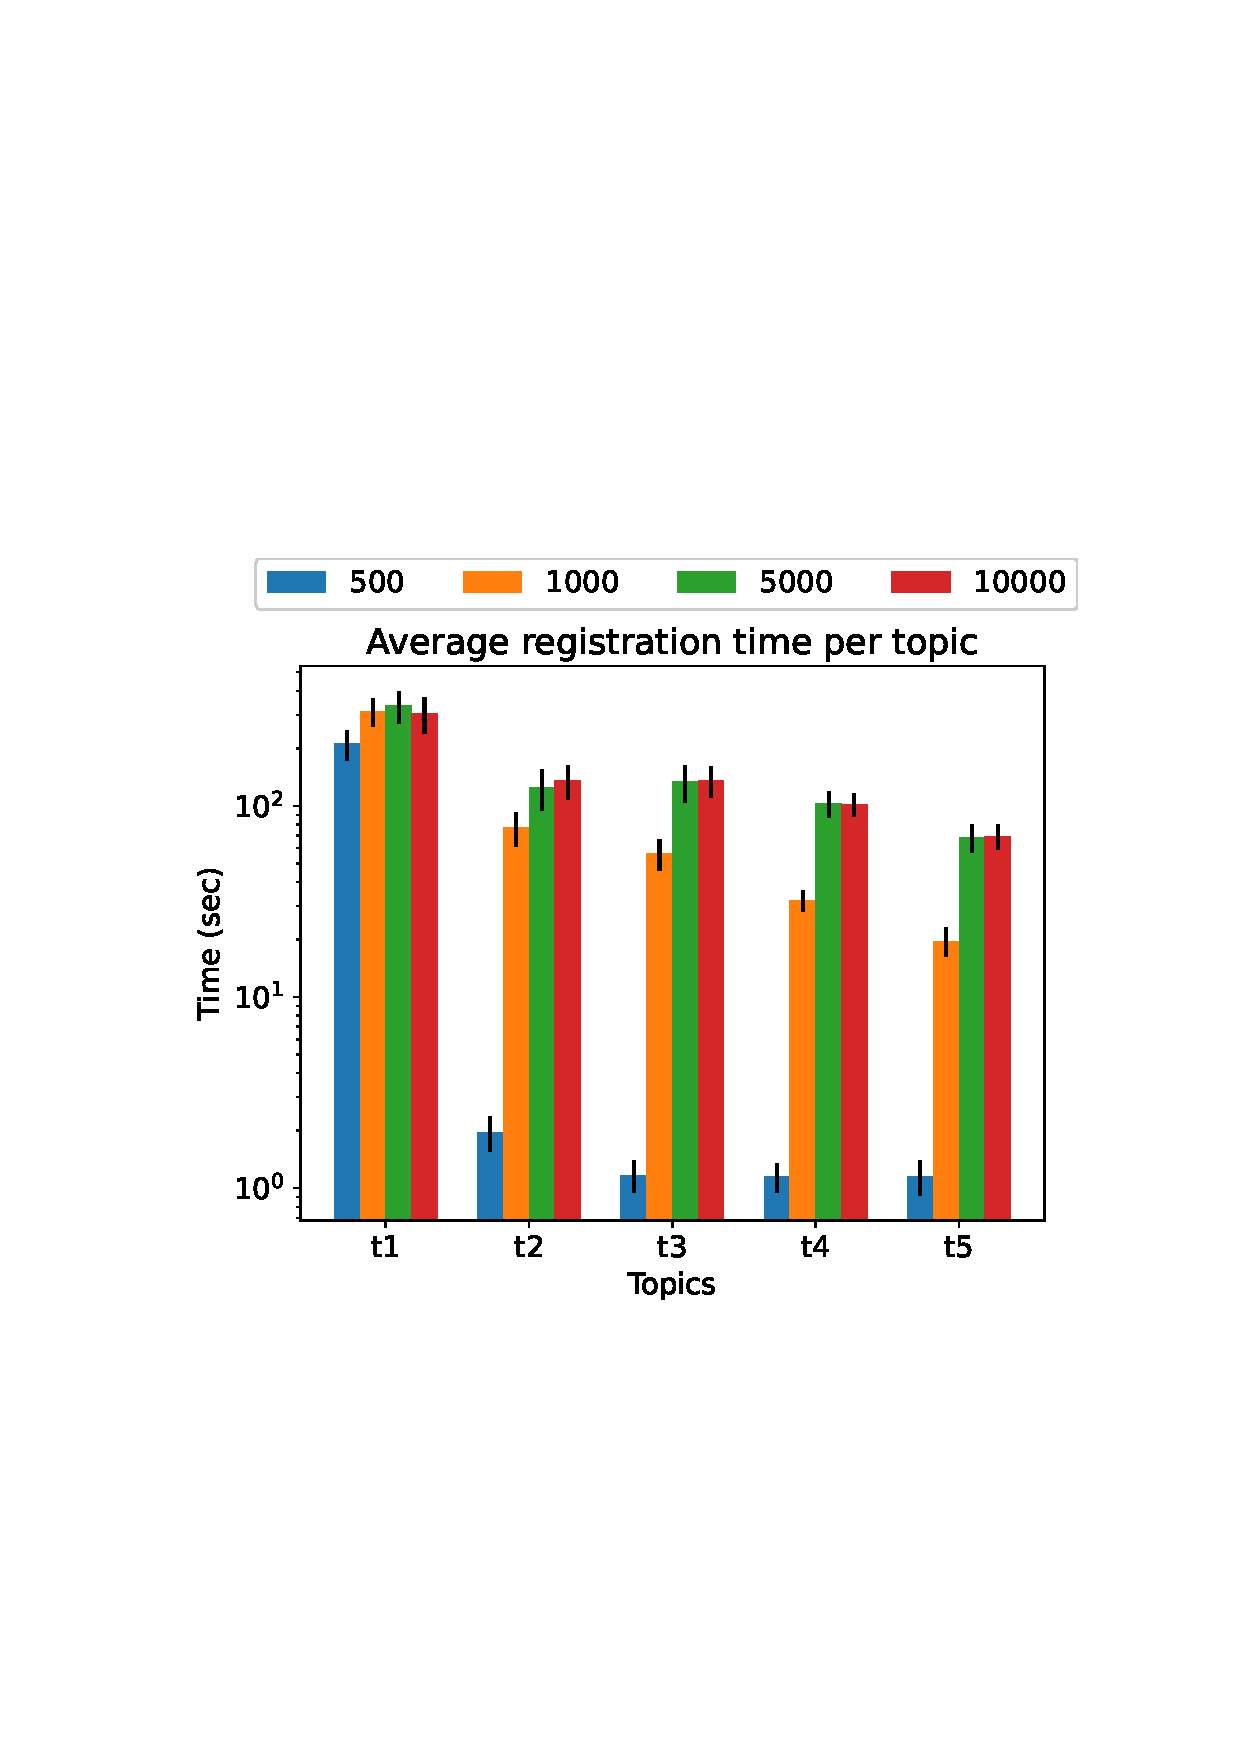
\includegraphics[width=0.225\textwidth]{img/eval/avg_time_register.png}
\label{fig:time_reg}
}
 \caption{Ticket registrations} 
\label{fig:registrations}
\vspace{-0.15in}
\end{figure}   

%\begin{figure}[h!]
%\centering
%%\epsfig{file=imgs/eval/scen5.pdf, width=0.45\textwidth}
%\includegraphics[width=0.225\textwidth]{img/eval/registration_origin.png}
%\caption{Registrations}
%\label{fig:regs}
%\vspace{-0.15in}
%\end{figure}

%\paragraph{\bf{Network load}:}
\sergi{TODO: change Log scale for fig \ref{fig:messages}}
In Figure~\ref{fig:messages}~and~\ref{fig:msg_distr} we can observe the traffic load generated in the network.
In Figure~\ref{fig:messages} we observe most of the messages are ticket requests/replies, and the subsequent registration request/replies
after receiving a ticket from a node. 
This is caused by the fact that nodes are constantly registering dynamically. 
In Figure~\ref{fig:msg_distr} the messages received distribution. 
We can observe some nodes receive much more messages.
This is caused by the bucket ndoe distributiong, where nodes with identifiers close to topic hash ids receive more initial tickets requests because there are less.
However, we can see the number of messages received does not exceed \hl{X} times the average value of the messages received. 
Moreover, we can also observe with the increase of nodes in the network, the load that these nodes receive does not increase in the same way. 
Therefore, the system is able to scale without danger of overloading some of the nodes of the network.

\begin{figure}[!h]
\centering
\subfigure[{Number of messages}]{
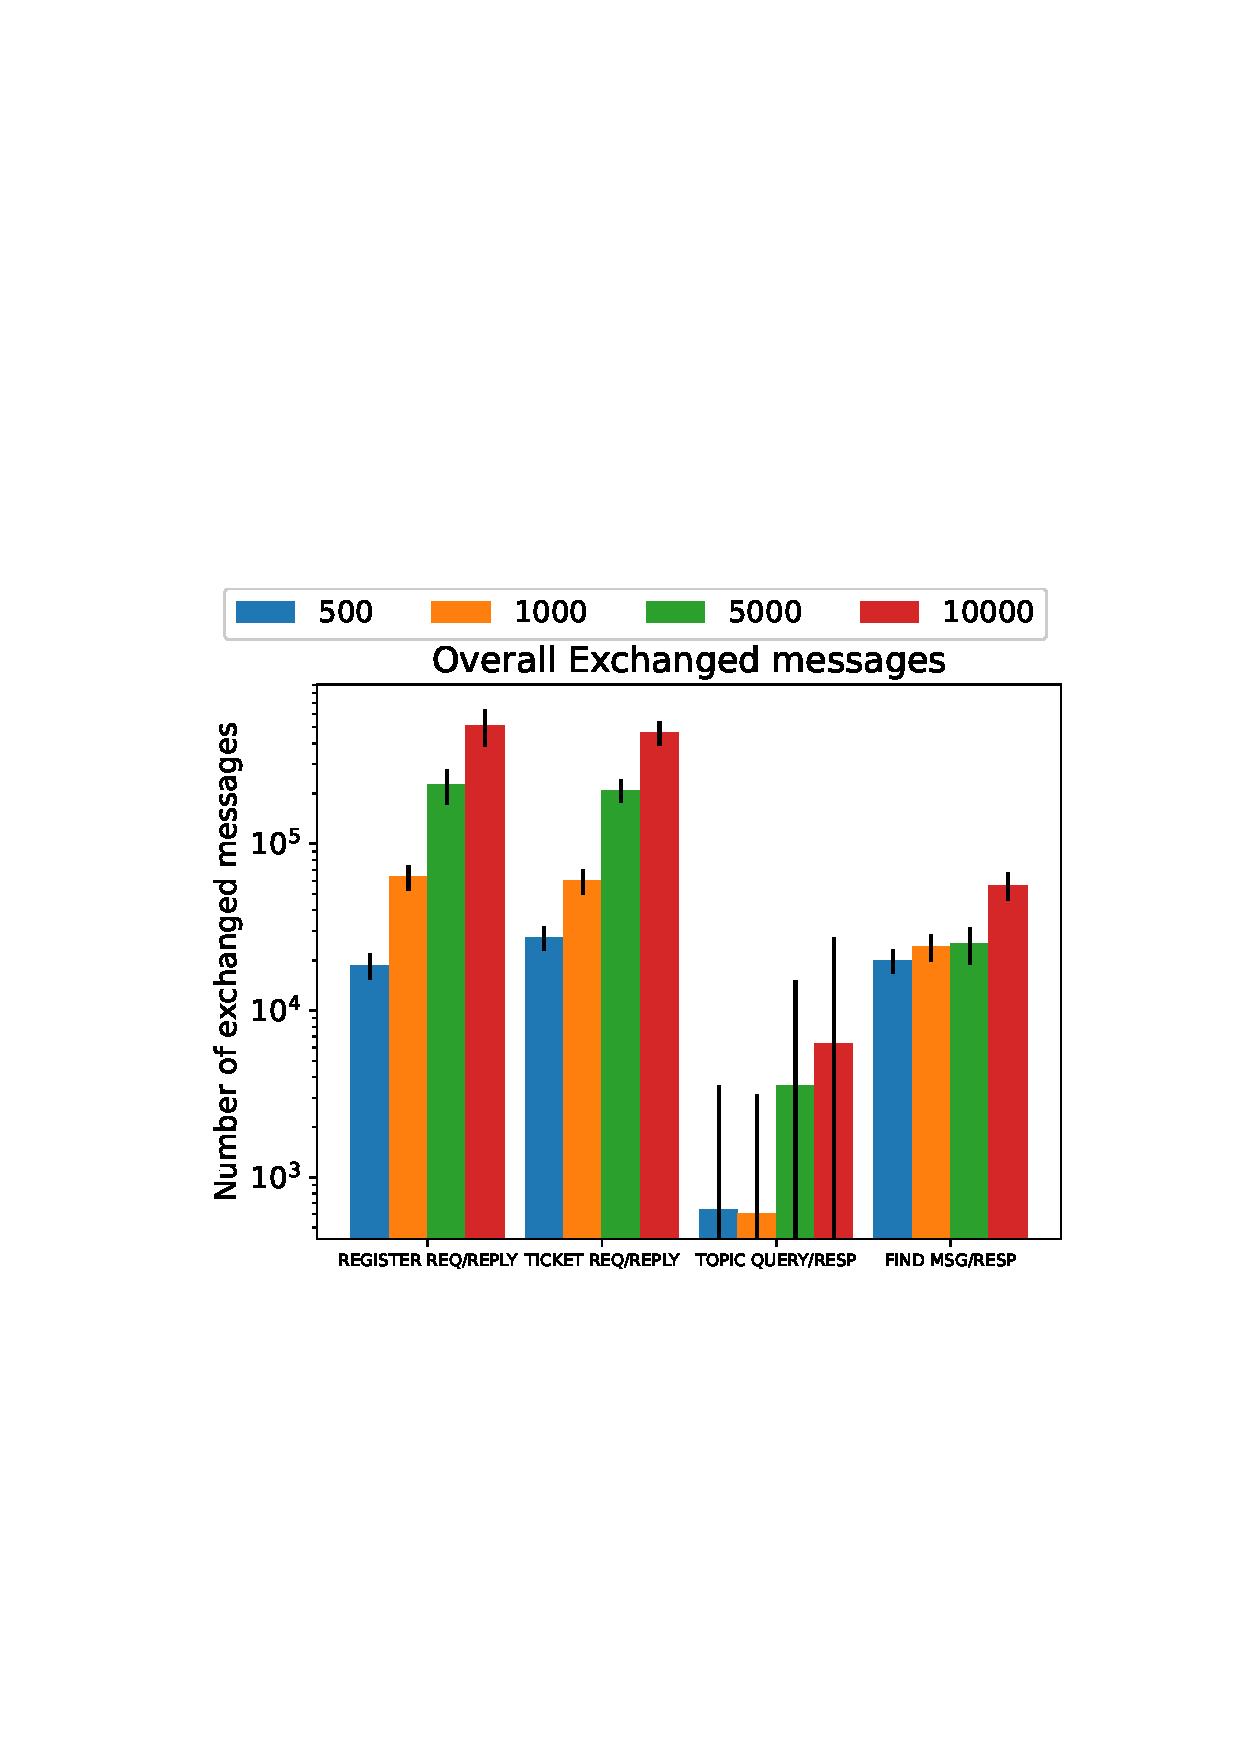
\includegraphics[width=0.225\textwidth]{img/eval/message_quantity.png} 
\label{fig:messages}
} 
\hspace{-0.25cm}
\subfigure[{Message distribution}]{
\includegraphics[width=0.225\textwidth]{img/eval/messages_received2.png} %\hspace{-1.5em}%
\label{fig:msg_distr}
}
 \caption{Traffic load} 
\label{fig:traffic}
\vspace{-0.15in}
\end{figure}   

%\paragraph{\bf{Discovery performance}:}

\sergi{TODO: modify figures with bigger fonts}

In Figure~\ref{fig:reg_disc}~and~\ref{fig:timedisc} we can observe how nodes are discovered within the network.
In Figure~\ref{fig:reg_disc} we observe the percentage of the nodes in the network that are discovered and how often are discovered.
Each node in the network is represented by a circle, and the size of the cirle represents the relative frequency of discoveries compared with other nodes in the network.
We can observe that for all topics the percentage of nodes discovered in the network is very close to 100\%. This means almost all nodes in the network are able to be discovered by other nodes. The number of dicovered nodes is not 100\% because of the existence of turbulence (there are some nodes just joined the network and there has not been enough time yet to be discovered). In case there are a low number of nodes for a specific topic (e.g. t5 with 500 nodes network) the 100\% is reached.
We can also observe Figure~\ref{fig:reg_disc} that the discovery distribution is bounded to \hl{X} times between the most discovered and the least discovered.
We observe the dots size are very regular and despite being not completely equal the differences are not substantial. 
In Figure~\ref{fig:timedisc} we observe the time between a registration is completed and the first time the registration
is returned in a lookup.
By observing this we can see how difficult is for a node to be discovered once is able to place a registration. 
We see the average time is between 20 and 10 seconds in most of the cases, except for the least popular topic t5 which is around 50\% higher. 
We also observe the deviation is bounded at around 60 seconds, with equivalent different for t5.


\begin{figure}[!h]
\centering
\subfigure[{Registrant discovery distribution}]{
\includegraphics[width=0.225\textwidth]{img/eval/registrant_distribution.png} 
\label{fig:reg_disc}
} 
\hspace{-0.25cm}
\subfigure[{Time between registration and first discovery}]{
\includegraphics[width=0.225\textwidth]{img/eval/min_time_discovery.png} %\hspace{-1.5em}%
\label{fig:timedisc}
}
 \caption{Discovery performance} 
\label{fig:discovery}
\vspace{-0.15in}
\end{figure}   


In Figure~\ref{fig:hopcount} we observe the hops necessary to traverse during a lookup to discover N distinct nodes for a topic.
In the simulation we set N to 50.
We observe the hopcount keeps quite stable between 20 and 40, even for the least popular topics where is more difficult to find registrations.

%TODO add lookup description including mechanisms to avoid sybils.

\begin{figure}[h!]
\centering
%\epsfig{file=imgs/eval/scen5.pdf, width=0.45\textwidth}
\includegraphics[width=0.35\textwidth]{img/eval/lookup_hopcount.png}
\caption{Lookup performance}
\label{fig:hopcount}
\vspace{-0.15in}
\end{figure}

\subsubsection{Sybil Attacks}

In the following we show the results of the performance evaluation of the discovery service under different sybil attacks.  The attacks that we evaluated in this section are of two types and are previously described in \hl{ref}. These attacks are eclipsing  and Denial-of-service (DoS) attacks.
Eclipsing attacks goal is to generate multiple fake identities within a topic to be able to eclipse existing nodes in the network.
Eclipsing a node imply all outbound and inbound connections are established to only sybil/fake nodes controlled by an attacker.
This allows the attacker to control the view of the network of the eclipsed node and can be used to co-opt a victim's mining power and use it to attack the blockchain's consensus algorithm.
DoS attacks instead is an attack meant to hamper the good performance or even to shut down the network, making it inaccessible to its intended users.  
In our case,  the goal of DoS attacks is to difficult or to block the discovery of nodes in the network and is specially important for topic with low popularity where finding all node in the network is very important.

In the implemented topic eclipsing attacks,  malicious nodes are sybil nodes that cooperate in order to eclipse other valid nodes.
Malicious and valid nodes have the same amount of bandwidth resources and malicious nodes respond to topic lookup requests and find messages with only other malicious nodes.
Malicious nodes also act as evil 'registrants' trying to place as much as registrations as possible by using bigger ticket size,  with malicious registrars attack, where evil registrars replies with only malicious nodes when receiving a topic query.

We implemented and evaluated two kind of DoS attacks.  
The first attack consists in a topic spam attack where a big number of sybil identities generated try to register for non-existing random topics.
By registering for non-existing topics,  evil nodes try to harm valid topics registrations, overflowing topic tables.
The second DoS attack consists on generating sybil identities that keep without replying when receiving valid nodes ticket requests or return very long waiting times. 
This way an attacker can try to backlog valid nodes ticket registrations.

In Figures~\ref{fig:reg_eclipse},~\ref{fig:discoverytime_eclipse}~and~\ref{fig:lookup_eclipse} we show performance results under a
topic eclipsing attack.
We compare results for topic eclipsing attacks targeted to the most popular topic (t1) and attacks targeted to the least popular topic (t5). 
In the simulation there are 2000 nodes, all of them participating in t1 and only 218 participating in t5. 
In the simulations there are an additional 20\% (400 in total) malicious nodes that target the specific topic and the number of resources used in the attack (IP addresses) vary from 1 address to 50.

\begin{figure}[!h]
\centering
\subfigure[{Active registrations eclipse attack t1 attack}]{
\includegraphics[width=0.22\textwidth]{img/eval/attack/registration_origin_t1.png} 
\label{fig:reg_eclipse_t1}
} 
\hspace{-0.15cm}
\subfigure[{Active registrations eclipse attack t5 attack}]{
\includegraphics[width=0.22\textwidth]{img/eval/attack/registration_origin_t5.png} %\hspace{-1.5em}%
\label{fig:reg_eclipse_t5}
}
 \caption{Active registrations under topic eclipsing attack} 
\label{fig:reg_eclipse}
\vspace{-0.15in}
\end{figure}   

In Figure~\ref{fig:reg_eclipse_t1} we observe the active registrations in the simulation per topic, for an eclipsing attack targeted to the most popular topic (t1), including active registrations of malicious nodes.
We can observe than even though the number of malicious nodes is equivalent to 20\%, the number of active registrations is lower than that. 
As expected, as the number of IP addresses used in the attack increaseas, the number of active registrations of malicious nodes also increase, since different malicious nodes with complete different IPs can not be diffierentiated from valid nodes.
For topic 5, the most vulnerable topic for being the least popular, we can observe a similar pattern of active registrations. 
However, we observe that despite malicious nodes being more (400 nodes) than valid nodes (218 nodes), active registrations of malicious nodes is kept lower than 30\% in all cases. Similarly to t1, the active registrations increase with the higher number of IPs used in the attack, since there is no way to a totally distributed attack without reusing IP addresses.


\begin{figure}[!h]
\centering
\subfigure[{Time between registration and first discovery t1 attack}]{
\includegraphics[width=0.225\textwidth]{img/eval/attack/min_time_discovery_t1.png} 
\label{fig:discoverytime_eclipse_t1}
} 
\hspace{-0.16cm}
\subfigure[{Time between registration and first discovery t5 attack}]{
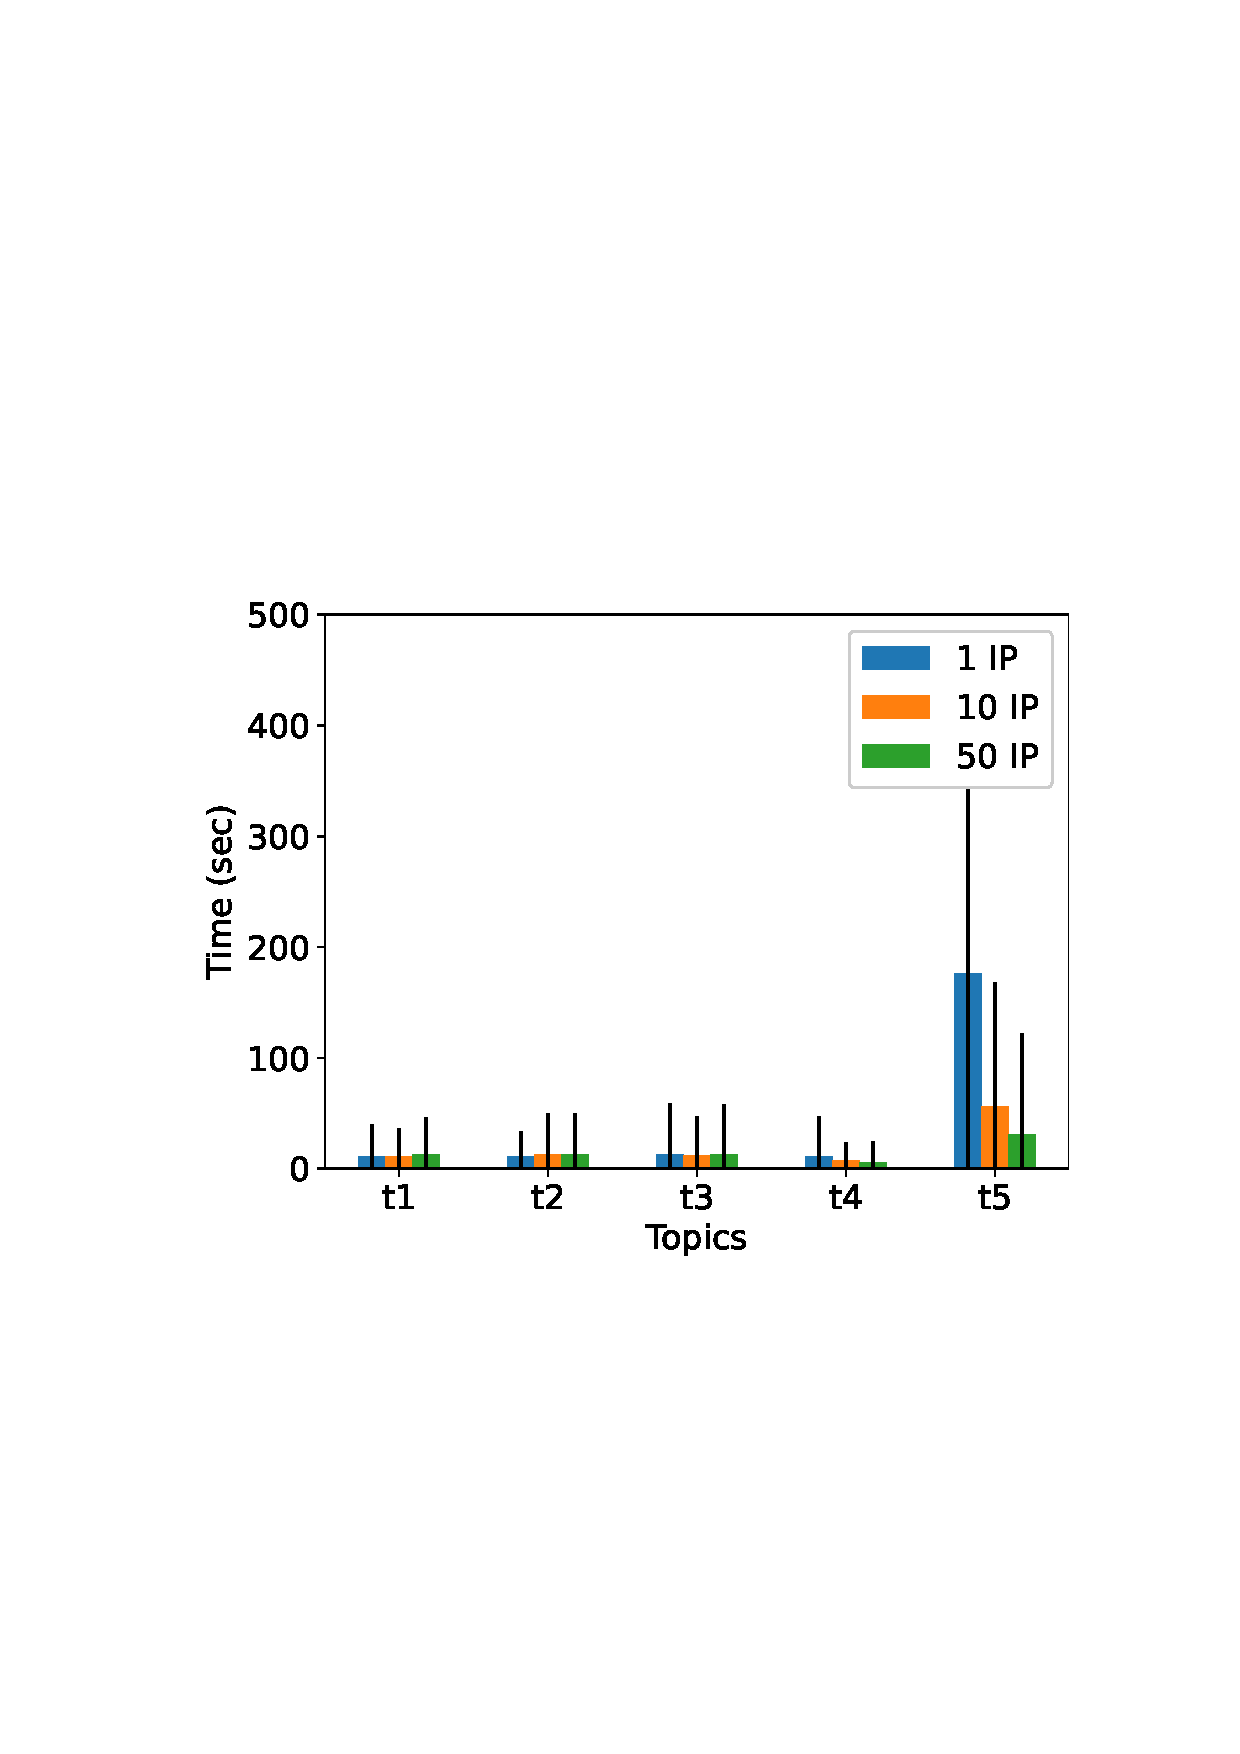
\includegraphics[width=0.225\textwidth]{img/eval/attack/min_time_discovery_t5.png} %\hspace{-1.5em}%
\label{fig:discoverytime_eclipse_t5}
}
 \caption{Time between registration and first discovery under topic eclipsing attack} 
\label{fig:discoverytime_eclipse}
\vspace{-0.15in}
\end{figure}   
\sergi{TODO: use same yaxis}

In Figure~\ref{fig:discoverytime_eclipse} we observe the average time between a node registers for a topic succesfully, and this node is discovered for the first time from the placed registration.
We can observe that when a topic is under attack the time required for first time discovery increases substantially.
\sergi{Not sure why discovery time is higher when using less ips in the attack, do we discard malicious nodes in the measurement?}

\begin{figure}[!h]
\centering
\subfigure[{Lookup hopcount eclipse attack t1}]{
\includegraphics[width=0.225\textwidth]{img/eval/attack/lookup_hopcount_t1.png} 
\label{fig:lookup_eclipse_t1}
} 
\hspace{-0.16cm}
\subfigure[{Lookup hopcount eclipse attack t5}]{
\includegraphics[width=0.225\textwidth]{img/eval/attack/lookup_hopcount_t5.png} %\hspace{-1.5em}%
\label{fig:lookup_eclipse_t5}
}
 \caption{Lookup hopcount under topic eclipsing attack} 
\label{fig:lookup_eclipse}
\vspace{-0.15in}
\end{figure}   

In Figure~\ref{fig:lookup_eclipse} we observe the lookup hopcount in the simulation per topic,  for an eclipsing attack targeted to the most popular topic (t1) and the least popular topic (t5).
\sergi{why lookup hopcount is worse for t5 with 1 ip than with 50 IPs. are malicious nodes taken into account?}

In Figure~\ref{fig:perf_spam} we observe the performance of the topic discovery system under  the topic spam attack.
In Figure~\ref{fig:active_regs_spam} we observe the average active registrations per topic increasing the number of Ip addresses used by sybil identities performing the attack.  
We observe that the number of registrations are  poorly affected by attackers. 
Only t1 seems to be affected.
\sergi{Why do registrations increase with more sybil ips for t1??}
In Figure~\ref{fig:time_register_spam} we observe the average time required for registering for a topic,  increasing the number of Ip addresses used by sybil identities performing the attack.  
We observe again it seems there is no substantial impact of the attack to the time required to register for each topic
In Figure~\ref{fig:time_discovery_spam} we observe the average time between and advertiser place a registration in a registrar and another node discovers it through the registrar,  increasing the number of Ip addresses used by sybil identities performing the attack.  
We observe again it seems there is no substantial impact of the attack, concluding the system is resistant to topic spam attacks.

\sergi{add spam storage used?}
\begin{figure*}[!h]
\centering
\subfigure[{Active registrations under topic spam attack}]{
\includegraphics[width=0.275\textwidth]{img/eval/attack/registration_origin_spam.png} 
\label{fig:active_regs_spam}
} 
\hspace{-0.16cm}
\subfigure[{Time to register under topic spam attack}]{
\includegraphics[width=0.275\textwidth]{img/eval/attack/avg_time_register_spam.png} %\hspace{-1.5em}%
\label{fig:time_register_spam}
}
\hspace{-0.15in}
\subfigure[{Time to first discovery topic spam attack}]{
\includegraphics[width=0.275\textwidth]{img/eval/attack/lookup_hopcount_spam.png} %\hspace{-1.5em}%
\label{fig:time_discovery_spam}
}
\label{fig:perf_spam}
\caption{Performance evaluation topic spam attack} 
\vspace{-0.15in}
\end{figure*}   

In Figure~\ref{fig:perf_dos} we observe the performance of the topic discovery system under the dos attack where registrars do not respond to advertisers trying to block active registrations.
In Figure~\ref{fig:active_regs_dos} we observe the average active registrations per topic increasing the number of sybil identites from 5\% to 20\% of the nodes in the network.
We observe that the number of registrations are affected by attackers, being more affected very popular topics,  but less affected low popularity topics.  However in none of the cases malicious nodes are able to block the active registrations and the reduction of the performance is lower than the number of sybils used.
In Figure~\ref{fig:time_register_dos} we observe the average time required for registering for a topic,  increasing the number of sybil identites from 5\% to 20\% of the nodes in the network.
We observe in this case it seems there is no substantial impact of the attack to the time required to register for each topic
In Figure~\ref{fig:time_discovery_dos} we observe the average time between and advertiser place a registration in a registrar and another node discovers it through the registrar,  increasing the number sybils again.
We also observe there is no substantial impact of the attack, concluding the system is resistant to DoS attacks.
\sergi{add spam storage used}

\begin{figure*}[!h]
\centering
\subfigure[{Active registrations under DoS attack}]{
\includegraphics[width=0.275\textwidth]{img/eval/attack/registration_origin_dos.png} 
\label{fig:active_regs_dos}
} 
\hspace{-0.16cm}
\subfigure[{Time to register under DoS attack}]{
\includegraphics[width=0.275\textwidth]{img/eval/attack/avg_time_register_dos.png} %\hspace{-1.5em}%
\label{fig:time_register_dos}
}
\label{fig:discovery_dos}
\hspace{-0.15in}
\subfigure[{Time to first discovery under DoS attack}]{
\includegraphics[width=0.275\textwidth]{img/eval/attack/min_time_discovery_dos.png} %\hspace{-1.5em}%
\label{fig:time_discovery_dos}
}
\label{fig:perf_dos}
\caption{Performance evaluation no-response DoS attack} 
\vspace{-0.15in}
\end{figure*}   


%\subsection{Testbed evaluation}
%
%"Geth"~\cite{go-ethereum} performance evaluation: \hl{TBC}.
